\subsection{Physical Layer}
\subsubsection{Overview}
The physical layer is primarily composed of an inverse kinematics verifier and a motion planner. Its main function is to verify the physical feasibility of transitions in the semantic solution proposed by the logic layer. It processes a semantic solution and returns either a success or a failure.
\begin{itemize}[]
	\item\textbf{Inverse Kinematics Verifier:} This module verifies whether the poses for grabbing and placing a module are possible from the current base position. If either pose is not feasible, the module attempts to find a base position that allows both poses. If both poses are feasible from the same base position, the verifier permits the semantic solution to proceed to the motion planner. If it fails to find such a position, it triggers an inverse kinematics failure and discards the semantic solution.
	
	\item\textbf{Motion Planner:} Upon receiving a transition, the motion planner determines a path from the start pose to the end pose that avoids collisions between the arm, the grabbed module, and other modules. If no collision-free path is found, the motion planner returns a motion planning failure, and discards the semantic solution.
\end{itemize}

\subsubsection{Inverse Kinematics Verifier}\label{IKDESIGN}
Inverse kinematics (IK) determines the joint angles required to position a mobile manipulator's end-effector at a desired location and orientation. There are two primary methods for solving IK \cite{IK}:
\begin{itemize}[]
	\item\textbf{Analytical Approach:} This method involves deriving a mathematical solution specific to each unique manipulator arm. It is complex because it requires detailed analysis and formulation. However, once the formulas are derived, calculations are extremely fast, making it suitable for frequent computations.
	
	\item\textbf{Pseudoinverse Jacobian Method}: This iterative method guesses the required joint angles and adjusts them incrementally to achieve the target position and orientation. It can be applied to any arm configuration without needing unique formulations but is computationally intensive.
\end{itemize}
Given the need for frequent IK calculations, the analytical approach is preferred. The mobile manipulator is represented using Denavit-Hartenberg (DH)\cite{DenavitHartenberg} parameters, which facilitates the derivation of analytical formulae for each joint. The formulae allow for efficient computation of IK, ensuring that the system can quickly verify and adjust the manipulator's poses.

\subsubsection{Manipulator Base Location Planning}
The mobile manipulator present in the MOSAR \cite{MOSAR} project can traverse the modular system. If the IK module fails to connect to a module from a position, moving the arm closer to the module that failed the inverse kinematic check could result in a successful solution like in figure \ref{basePlanning}. When the inverse kinematics module fails a check, it attempts to move the base to another available surface in between the 2 movement points. As our available arm is stationary, our implementation will only include base location planning if time permits.
\begin{figure*}[h]
	\centering
	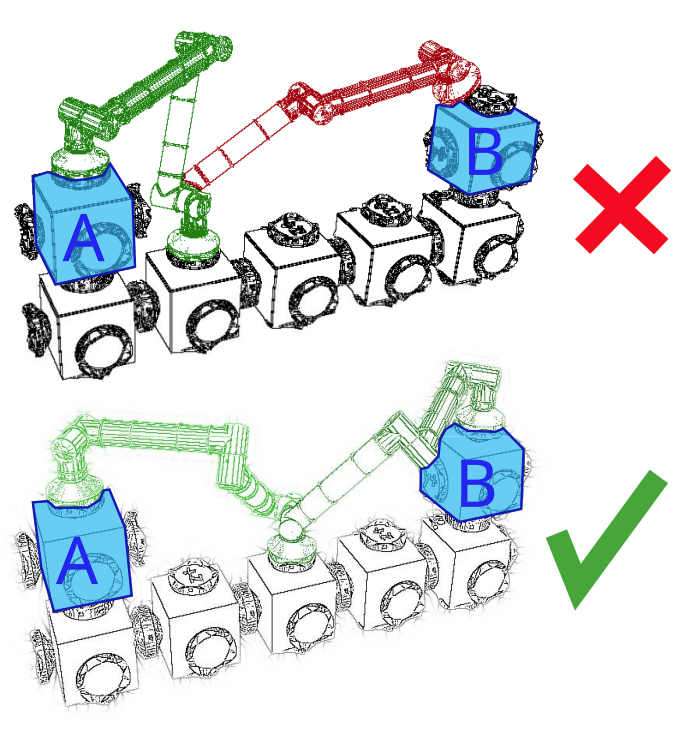
\includegraphics[width=0.5\textwidth]{basePlanning.png}
	\caption{Inverse kinematic checks performed to verify if it is
		possible to translate a module from position A to position B.
		In the first case (above) this is not possible, but it is solved
		by changing the intermediate position in the second case
		(bottom). Image and text from \cite{9438257}}
	\label{basePlanning}
\end{figure*}

\subsubsection{Motion Planning}
Originally, the plan was to implement a motion planner using the Rapidly-exploring Random Tree (RRT) algorithm used here \cite{8412538} to generate collision-free motion paths for the robot arm. However, due to time constraints, a simpler approach is adopted.
\\\\
In the lab scenario, where modules are reconfigured on a platform by a stationary robot arm, motion planning is simplified. We can assume that a module can be picked up if there are no modules above it and if it is within reach according to the inverse kinematic solution. Modules are then moved between positions by lifting them to the arm's maximum z-limit, moving above the new position, and lowering them into place.
\\\\
Additional physical constraints are applied through feedback:
\begin{itemize}[]
	\item Modules cannot be moved to negative-z values due to the platform.
	\item Modules must be placed on top of the platform or another module due to gravity.
\end{itemize}
These constraints will induce physical layer failures, leading to an expected increase in the time taken to generate results compared to operation in space.

\subsubsection{Failure Feedback}
The physical layer reports various types of failures upon detecting conflicts, including:
\begin{itemize}[]
	\item\textbf{Out of reach:} The starting and final positions of the module are unreachable for the current mobile manipulator.
	\item\textbf{No Base Location:} Although the starting and final positions of the module are within reach, there is no suitable base position on the module configuration to reach both points.
	\item\textbf{Collision:} There is no available path to move the module without colliding with another module.
\end{itemize}

